% =============================================================================
%  MIRROR - Multimodal Intelligent Radiology Reasoning and Observation Reporter
%  SSRN preprint (v9): accuracy revision. The post-hoc invariance check is
%  demoted from a headline result to a regression test; the operating point and
%  the calibration baseline are reported directly; the hosted vision-LLM engine
%  is separated from the benchmarked local PyTorch stack wherever a figure or a
%  claim depends on which one produced it. Max 8 pages.
%
%  HOW TO USE: compiles in Overleaf or any TeX install (engine: pdfLaTeX) in a
%  SINGLE pass; the architecture figure and the result graph are drawn inline
%  (TikZ/pgfplots), the tables are inlined, and the bibliography is embedded (no
%  bibtex step). The only external assets are the three UI screenshots in
%  paper/figures/*.png; upload that folder alongside this file. Each screenshot
%  is guarded by \IfFileExists, so the document still compiles (with a red
%  placeholder box) if the images are missing.
%
%  Every number in this paper traces to a committed JSON under results/ or to
%  paper/calibration_baseline.py. See paper/REVISION-NOTES-v9.md for the map.
% =============================================================================
\documentclass[10pt,twocolumn]{article}

\usepackage[margin=0.85in]{geometry}
\usepackage{times}
\usepackage{microtype}
\usepackage{graphicx}
\usepackage{booktabs}
\usepackage{array}
\usepackage{amsmath}
\usepackage{amssymb}
\usepackage{enumitem}
\usepackage{xcolor}
\usepackage{caption}
\usepackage{tikz}
\usepackage{pgfplots}
\pgfplotsset{compat=1.18}
\usepackage[colorlinks=true,allcolors=blue!55!black]{hyperref}
\usepackage{url}
\usepackage{placeins}   % \FloatBarrier: keep floats from drifting into later sections
\usetikzlibrary{arrows.meta,positioning}

% Give LaTeX more room to place the many two-column-wide floats before it gives up
% and defers them to the end (which is what pushed Table/Figure into the
% references). These loosen the default "a float page must be 50% full" etc. limits.
\renewcommand{\topfraction}{0.9}
\renewcommand{\bottomfraction}{0.9}
\renewcommand{\textfraction}{0.08}
\renewcommand{\floatpagefraction}{0.7}
\setcounter{topnumber}{3}
\setcounter{totalnumber}{5}

\newcommand{\code}[1]{\texttt{\small #1}}

% ---- Compile even without the screenshot files -------------------------------
% #1 = path, #2 = width, #3 = fallback caption text.
\newcommand{\figorbox}[3]{%
  \IfFileExists{#1}{\includegraphics[width=#2]{#1}}%
  {\fbox{\parbox[c][2.8cm][c]{#2}{\centering\color{gray}\itshape #3\\(add image to paper/figures/)}}}}

\definecolor{mirrorblue}{RGB}{31,86,145}
\definecolor{mirrorgray}{RGB}{90,96,104}
\definecolor{boxbg}{RGB}{237,243,250}

\captionsetup{font=small,labelfont=bf}

\title{MIRROR}   % for PDF metadata only; the visible title block is built below
\hypersetup{pdftitle={MIRROR: Multimodal Intelligent Radiology Reasoning and Observation Reporter},
            pdfauthor={Vignesh Nagarajan}}

\begin{document}

% =============================================================================
%  Title block spans both columns.
% =============================================================================
\twocolumn[{%
\centering
\vspace{6pt}
{\Huge\bfseries MIRROR}\\[6pt]
{\large\bfseries Multimodal Intelligent Radiology Reasoning and Observation Reporter}\\[10pt]
{\itshape\normalsize A three-layer radiology pipeline whose language layer reads
structured evidence rather than pixels; three modality taxonomies are registered
and routed, one of which, chest X-ray, is trained and benchmarked here.}\\[18pt]

% ---- Two authors, side by side, each in a fixed-width box so the long
%      affiliation lines wrap inside their column; the shared GIST internship
%      affiliation sits on one centered line beneath both author blocks. ----
\normalsize
\begin{minipage}[t]{0.45\textwidth}
\centering
{\large\textbf{Vignesh Nagarajan}}\\[3pt]
{\small\itshape Corresponding Author}\\[4pt]
{\small Brown Foundation Scholar, Texas A\&M University}\\[2pt]
{\small Department of Computer Science \& Engineering}\\[2pt]
{\small\texttt{vigneshn26@tamu.edu}}
\end{minipage}%
\hspace{0.06\textwidth}%
\begin{minipage}[t]{0.45\textwidth}
\centering
{\large\textbf{Sriram Venkatapathy}}\\[3pt]
{\small\itshape Research Mentor}\\[4pt]
{\small Applied AI Researcher, Capital One}\\[2pt]
{\small PhD in Computer Science, IIT Hyderabad}\\[2pt]
{\small\texttt{sriram.venkatapathy@gmail.com}}
\end{minipage}\\[14pt]
{\small Global Indian Scientists \& Technocrats (GIST) 2026 Summer Research Internship}\\[20pt]

\begin{minipage}{0.88\textwidth}
\small
\textbf{Abstract.}
Most medical-imaging models stop at a prediction, offering neither the location of
the evidence nor an account a clinician can read. We present \textbf{MIRROR}, a
three-layer radiology pipeline composing a multi-label classifier,
class-activation evidence localization, and a report generator that receives only
structured upstream evidence: a per-label probability, a present/absent flag, and
a saliency-derived anatomical region. Because the language layer never receives
the image, the report cannot assert a finding the classifier did not produce. That
guarantee is \emph{finding-level, not detail-level}: the descriptive prose framing
each finding is generated text, is not checked against the image, and we give a
worked example in which it is measurably ungrounded. One registry supplies the
taxonomy, anatomical vocabulary, and report phrasing for chest X-ray (14
findings), brain MRI (11), and head CT (11), with routing explicit or read from
the DICOM modality tag; all three are exercised by the test suite, and one, chest
X-ray, is trained and benchmarked. On ChestMNIST, a downsampled ChestX-ray14
derivative with the identical 14-label taxonomy, a DenseNet-121 reaches macro
AUROC $0.729$ ($95\%$ CI $[0.718,0.738]$) with a per-label ordering that tracks
finding visibility. At the default $0.5$ threshold that same model emits no
positive prediction whatsoever for $11$ of the $14$ labels, and macro F1 is
$0.031$. Its calibration nonetheless looks excellent (Brier $0.045$, ECE
$0.018$), yet a constant predictor that ignores the image and always returns each
label's base rate scores macro Brier $0.047$ on the same test set. We report this
as a finding: under heavy multi-label class imbalance, aggregate calibration
metrics are close to uninformative, and a model silent on most of its taxonomy
still posts excellent-looking ones. All headline numbers carry bootstrap $95\%$
confidence intervals and every run stamps a reproducibility record.
\end{minipage}
\vspace{10pt}
}]

% -----------------------------------------------------------------------------
% -----------------------------------------------------------------------------
\section{Introduction}

Deep networks now match specialists on narrow chest-radiograph reading
tasks~\cite{rajpurkar2017chexnet}, yet clinical adoption remains limited by a
trust gap: a bare probability tells a radiologist neither \emph{where} the model
is looking nor \emph{why} it concluded what it did, and high-stakes decisions
demand models that can be interrogated~\cite{rudin2019stop}. Saliency methods such
as Grad-CAM~\cite{selvaraju2017gradcam} expose \emph{where} a prediction comes
from, and language models can render structured evidence as prose, but the two are
rarely composed into one system whose outputs stay mutually consistent.

\textbf{MIRROR} composes them: image $\rightarrow$ prediction $\rightarrow$
localization $\rightarrow$ reasoning $\rightarrow$ report. Its central constraint
is \emph{grounding}: the language layer receives only the structured evidence
produced upstream (labels, probabilities, named saliency regions), never the raw
image, so the report can assert only findings the classifier predicted and the
localizer situated. Only the finding taxonomy, the anatomical vocabulary, and a
little report phrasing differ between modalities, so these are centralized in one
registry and a study is routed to the correct classifier head explicitly or from
its DICOM modality tag.

\paragraph{Research question.} Can a radiology pipeline be built so that its
language layer is structurally incapable of asserting a finding the classifier did
not detect, and what does that constraint cost? We answer the first half
architecturally and the second empirically, on chest radiographs. Two things this
paper does \emph{not} answer should be stated at the outset. It does not measure
explanation \emph{quality}: our harness defines a pointing-game and IoU protocol
against the NIH lesion boxes, but running it needs a checkpoint trained on the
full-resolution release, so no box-level score is reported here and none should be
inferred. Nor does it measure whether any of this helps a human, which would need
a reader study with radiologists timed and scored on the same studies with and
without the explanation and report layers.

\paragraph{Contributions.}
\begin{enumerate}[leftmargin=1.4em,itemsep=1pt]
  \item The distinction between \emph{finding-level} grounding, which constraining
  the language layer to structured evidence does buy and which is checkable, and
  \emph{detail-level} grounding, which it does not buy and which we show failing
  in a real generated report.
  \item A registry-driven multimodality in which a modality's taxonomy, anatomical
  vocabulary, and report phrasing are data rather than code. Three taxonomies are
  registered, routed, and exercised by the test suite; one is benchmarked.
  \item An open-source implementation: three backbones, two explainability
  methods, an LLM report backend with a deterministic offline fallback, a real
  DICOM ingest, and two very different inference engines behind one response
  contract (Fig.~\ref{fig:ui}).
  \item Two negative results the harness surfaces on our own model: silence across
  most of the label set at the default threshold, and aggregate calibration metrics
  that barely separate a trained classifier from a constant.
\end{enumerate}

% -----------------------------------------------------------------------------
\section{Literature Review}
\label{sec:litreview}

\paragraph{Classification and visual explanation.} The NIH ChestX-ray8/14
release~\cite{wang2017chestxray} ($112{,}120$ frontal radiographs, 14 pathologies)
made supervised deep learning on this modality practical, and
MIMIC-CXR~\cite{johnson2019mimiccxr} added paired free-text reports.
CheXNet~\cite{rajpurkar2017chexnet} showed a 121-layer
DenseNet~\cite{huang2017densenet} reaching radiologist-level pneumonia detection;
EfficientNet~\cite{tan2019efficientnet} and Vision
Transformers~\cite{dosovitskiy2021vit} complete the standard toolkit, and MIRROR
keeps all three interchangeable with DenseNet-121 primary. On the explanation
side, Grad-CAM~\cite{selvaraju2017gradcam} localizes the evidence behind a CNN
prediction via gradients and Score-CAM~\cite{wang2020scorecam} removes the
gradient dependence. The pointing-game protocol~\cite{zhang2016pointing} and IoU
against annotated lesions turn heatmaps into quantitative scores; our harness
implements both, though we do not run them here.

\paragraph{Critiques of post-hoc explanation.} Adebayo et
al.~\cite{adebayo2018sanity} showed several saliency methods can be insensitive to
the model and the data they purport to explain, and argued for sanity checks
before any map is trusted. Rudin~\cite{rudin2019stop} argued more sharply that
high-stakes decisions call for inherently interpretable models rather than
post-hoc explanations of black boxes. MIRROR is squarely the kind of system these
critiques target, and we take up its position against them in
Section~\ref{sec:discussion} rather than citing them as background.

\paragraph{Report generation.} Systems emitting radiology prose range from
TieNet~\cite{wang2018tienet} to memory-driven transformers such as
R2Gen~\cite{chen2020r2gen} to decoders optimized for factual
correctness~\cite{liu2019clinically}. The recurring failure mode is
hallucination: prose generated directly from pixels can assert findings the model
never detected. Surveys of medical XAI~\cite{tjoa2021survey} note that
interpretability and report generation are usually studied separately. MIRROR's
contribution is neither a new classifier nor a new saliency method but their
composition under a constraint that bounds what the report may assert.

% -----------------------------------------------------------------------------
\section{System Architecture}
\label{sec:method}

MIRROR chains three layers; each layer's output is the grounded input to the next
(Fig.~\ref{fig:arch}).

\begin{figure}[tbp]
\centering
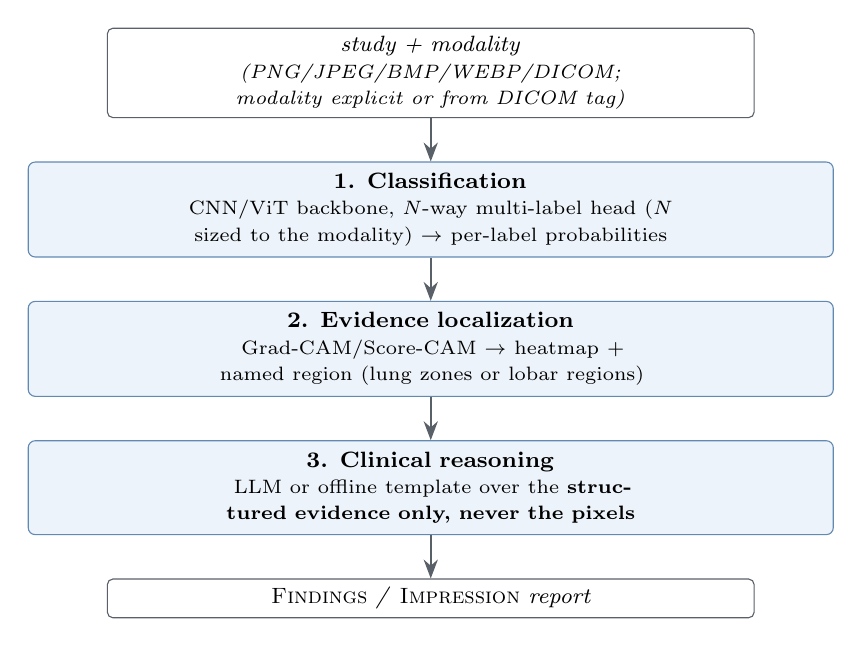
\begin{tikzpicture}[
  node distance=5.5mm,
  layer/.style={rectangle, rounded corners=2.5pt, draw=mirrorblue!70, fill=boxbg,
                text width=0.82\linewidth, align=center, inner sep=4pt,
                font=\footnotesize},
  io/.style={rectangle, rounded corners=2pt, draw=mirrorgray, fill=white,
             text width=0.66\linewidth, align=center, inner sep=3pt,
             font=\footnotesize\itshape},
  arr/.style={-{Stealth[length=2.4mm]}, thick, mirrorgray}
]
\node[io] (img) {study + modality \\ \scriptsize(PNG/JPEG/BMP/WEBP/DICOM;
   modality explicit or from DICOM tag)};
\node[layer, below=of img] (clf)
  {\textbf{1. Classification}\\ \scriptsize CNN/ViT backbone, $N$-way multi-label
   head ($N$ sized to the modality) $\rightarrow$ per-label probabilities};
\node[layer, below=of clf] (loc)
  {\textbf{2. Evidence localization}\\ \scriptsize Grad-CAM/Score-CAM
   $\rightarrow$ heatmap + named region (lung zones or lobar regions)};
\node[layer, below=of loc] (rep)
  {\textbf{3. Clinical reasoning}\\ \scriptsize LLM or offline template over the
   \textbf{structured evidence only, never the pixels}};
\node[io, below=of rep] (out) {\textsc{Findings} / \textsc{Impression} report};
\draw[arr] (img) -- (clf);
\draw[arr] (clf) -- (loc);
\draw[arr] (loc) -- (rep);
\draw[arr] (rep) -- (out);
\end{tikzpicture}
\caption{The MIRROR pipeline as deployed in the local PyTorch stack, which is the
configuration benchmarked in Section~\ref{sec:results}. Layers 2 and 3 are
individually toggleable, which recovers the conditions of
Section~\ref{sec:setup}. The hosted engine of Section~\ref{sec:serving} does not
have this structure.}
\label{fig:arch}
\end{figure}

\subsection{Layer 1: Classification}
The classifier is a factory over three ImageNet-pretrained backbones: DenseNet-121
(default), EfficientNet-B0, and ViT-B/16, with a multi-label head whose width $N$
is the size of the active modality's taxonomy (14 for chest X-ray, 11 each for
brain MRI and head CT; sigmoid applied at loss and inference time, so the network
emits raw logits). Inputs are resized to the backbone's $224\times224$ input and
normalized with ImageNet statistics. Training uses \code{BCEWithLogitsLoss},
AdamW, a cosine schedule, and dropout $0.2$, selecting on best validation macro
AUROC.

\paragraph{DICOM ingest.} Real radiology data arrives as DICOM, and the gap
between that and a PNG is not a file-format detail. Stored pixel values are not
display values: they must pass through the modality LUT (rescale slope and
intercept, which is what turns raw CT counts into Hounsfield units) and then the
VOI or window LUT that selects the diagnostic contrast range, and a
\code{MONOCHROME1} photometric interpretation means the stored values are inverted
relative to the usual convention. Skipping any of these silently trains a model on
images no radiologist would recognize, most visibly on \code{MONOCHROME1} studies,
which arrive as photographic negatives of what they should be. MIRROR ships an
ingest that applies all three before the pipeline sees a pixel, lifts only non-PHI
technical tags, and exposes the modality tag for routing.

\subsection{Layer 2: Evidence Localization}
For each positive label (top-$k$, $k{=}3$ by default, to bound compute), this layer
computes a class-activation map, either Grad-CAM (forward/backward hooks on a
per-backbone target layer) or Score-CAM (gradient-free); ViT maps are recovered by
reshaping the patch-token sequence back to a $14\times14$ grid. The activated
region's centroid is mapped into a $3\times3$ anatomical grid in radiology
convention (patient-right on the viewer's left), with the modality's plane picking
the vocabulary: lung zones for a frontal chest film, lobar regions for an axial
brain-MRI or head-CT slice.

\subsection{Layer 3: Clinical Reasoning}
This layer converts structured evidence (labels, probabilities, named regions) into
a \textsc{Findings}/\textsc{Impression} report via a system prompt plus an
evidence-grounded user prompt with per-label plain-English glosses. The backend is
an LLM (Claude) at low temperature, with a deterministic offline template fallback
on any error, so the system yields a coherent report with no network or API key.
Predictions below the confidence threshold ($0.5$) surface as pertinent negatives
rather than being dropped. Because both backends consume identical evidence,
swapping them changes \emph{how fluently} the report reads, not which findings it
asserts; and because the layer never receives the image, it cannot introduce
findings absent from the upstream evidence. The grounding is therefore at the
level of findings, not of the prose framing them, a distinction that carries most
of this paper's argument (Section~\ref{sec:discussion}).

\subsection{Multi-modality via a modality registry}
Swapping a chest radiograph for a brain MRI or head CT changes only the taxonomy
the head predicts, the vocabulary a saliency centroid is named in, and a little
report phrasing (so a normal brain study reads ``no acute intracranial
abnormality,'' not ``no acute cardiopulmonary abnormality''). These live in one
registry (Table~\ref{tab:modalities}), the single source of truth for each
modality's labels, glosses, plane, and report guidance; a hand-kept TypeScript
mirror gives the hosted engine and UI the identical taxonomy and \emph{ordering}
(output index $i$ maps to $\text{labels}[i]$). Modality is resolved explicitly or,
for DICOM, from the (0008,0060) tag, and the orchestrator caches one engine per
modality on demand. The claim is architectural and scoped as such: routing, head
sizing, vocabulary, and phrasing are exercised by the test suite for all three
taxonomies, but no brain-MRI or head-CT checkpoint has been trained, so MIRROR
makes no predictive claim on those modalities.

\begin{table}[tbp]
\centering
\caption{The modality registry. Registration means routing, head sizing, and
anatomical vocabulary are implemented and tested. Only chest X-ray is trained and
benchmarked here.}
\label{tab:modalities}
\footnotesize
\begin{tabular}{@{}p{0.20\linewidth}rp{0.30\linewidth}p{0.22\linewidth}@{}}
\toprule
\textbf{Modality} & \textbf{\#lbl} & \textbf{Taxonomy source} & \textbf{Location vocab.} \\
\midrule
Chest X-ray & 14 & NIH ChestX-ray14 & lung zones (frontal) \\
Brain MRI   & 11 & Brain Tumor MRI + neuro findings & lobar regions (axial) \\
Head CT     & 11 & RSNA ICH subtypes + acute findings & lobar regions (axial) \\
\bottomrule
\end{tabular}
\end{table}

\subsection{Orchestration and serving}
\label{sec:serving}
A single \code{analyze()} entry point runs the stages, records per-stage timings,
and returns one result object; layers 2 and 3 are individually toggleable. Two
engines satisfy the same JSON contract (Table~\ref{tab:topology}), so the web UI
(Fig.~\ref{fig:ui}) is identical either way: a finding carries \emph{either} a
rendered Grad-CAM overlay (local) \emph{or} a normalized bounding box (hosted).

The two engines are not two implementations of one design, and the difference
matters for every claim here. The local stack is the architecture of
Fig.~\ref{fig:arch}. The hosted engine exists because that stack does not fit
serverless limits, and replaces the whole thing with a single vision LLM under a
forced tool call returning the per-label probabilities, one box per present
finding, and the report in one response. That engine reads pixels directly, so
MIRROR's grounding constraint \textbf{does not hold on the hosted path}: nothing
structurally prevents its prose from asserting a finding its own probability
vector does not support. Everything benchmarked in Section~\ref{sec:results} is
the local stack, and hosted-engine figures are labelled as such.

\begin{figure*}[tp]
\centering
\figorbox{figures/ui-predictions.png}{0.52\textwidth}{MIRROR reading-room UI screenshot}
\caption{The MIRROR ``reading-room'' web UI, showing a session on the
\textbf{hosted serverless engine}, where a vision LLM reads the image directly and
returns probabilities, boxes, and report text. This is \emph{not} the benchmarked
DenseNet-121 local stack, and no number in this figure is a measured result: it
illustrates the interface and the response contract only. A chest radiograph is
uploaded with the indication \emph{``productive cough, 3 days,''} all 14
ChestX-ray14 labels are scored, and findings above threshold surface with a
location. Both engines drive this identical interface.}
\label{fig:ui}
\end{figure*}

\begin{table}[tbp]
\centering
\caption{Two inference engines behind one response contract. Only the local stack
implements the grounded architecture of Fig.~\ref{fig:arch}, and only it is
benchmarked here.}
\label{tab:topology}
\footnotesize
\begin{tabular}{@{}p{0.24\linewidth}p{0.32\linewidth}p{0.30\linewidth}@{}}
\toprule
 & \textbf{Local stack} & \textbf{Hosted (serverless)} \\
\midrule
Engine        & FastAPI + PyTorch     & Next.js route, vision LLM \\
Classify      & DenseNet/EffNet/ViT   & LLM scores $N$ labels \\
Localize      & Grad-CAM/Score-CAM PNG & LLM returns a bbox \\
Report        & LLM or template       & LLM, same call \\
Sees pixels?  & Layer 1 only          & Every stage \\
Inputs        & \small +DICOM, BMP    & PNG/JPEG/WEBP \\
\bottomrule
\end{tabular}
\end{table}

% -----------------------------------------------------------------------------
\section{Experimental Setup}
\label{sec:setup}

\paragraph{Data.} MIRROR targets NIH ChestX-ray14~\cite{wang2017chestxray}
($112{,}120$ radiographs, 14 multi-label pathologies). Because the full release is
$45$~GB and needs a GPU, we evaluate on \textbf{ChestMNIST}~\cite{yang2023medmnist},
its downsampled derivative in MedMNIST~v2 (CC~BY~4.0), which carries the
\emph{identical} 14-label taxonomy in the identical order, so MIRROR runs on it
unchanged. We sample $8{,}000$ studies from the pooled official train and
validation splits and hold out $10\%$, giving $7{,}200$ training and $800$
validation images, and evaluate on $12{,}000$ held-out test images. Training is
DenseNet-121 on CPU, AdamW at learning rate $3\times10^{-4}$, weight decay
$10^{-5}$, batch $32$, best of a four-epoch run on validation macro AUROC. Source
images are $64\times64$ and are \emph{upsampled} to the backbone's $224\times224$
input: there is no genuine $224$-pixel information anywhere in this experiment,
and findings whose radiographic signature is a few millimetres wide are largely
destroyed before training begins.

\paragraph{Metrics.} \emph{Discrimination:} per-label and macro AUROC, and macro
AUPRC. \emph{Operating point:} sensitivity, specificity, PPV, and NPV at the $0.5$
threshold, the quantities a clinician reads off a model. \emph{Calibration:} Brier
score and Expected Calibration Error ($10$ equal-width bins). Each headline metric
carries a bootstrap $95\%$ confidence interval: the test set is resampled with
replacement $B{=}1000$ times, a \emph{single} resample driving all metrics so the
intervals are mutually consistent, reported as two-sided percentile intervals
($\alpha{=}0.05$).

\paragraph{Post-hoc regression test.} Three conditions,
\code{classification\_only}, \code{with\_localization}, and \code{full\_mirror},
run the same studies with layers 2 and 3 switched on and off. Those layers modify
no weights and no logits, so the predictions must be identical across conditions;
the harness verifies this and profiles the per-stage wall-clock cost of each added
layer. This is a test that the implementation matches the design, not an
experiment with an uncertain outcome, and Section~\ref{sec:ablation} reports it as
such. Every results file stamps a reproducibility record (seed, git commit,
library versions).

% -----------------------------------------------------------------------------
\section{Results}
\label{sec:results}

Every number below is measured on this machine with the local PyTorch stack and
traces to a JSON committed in the repository.

\subsection{Discrimination on ChestMNIST}
\label{sec:chestmnist}
The DenseNet-121 reaches macro AUROC $0.729$ (bootstrap $95\%$ CI
$[0.718,0.738]$) on the $12{,}000$-image test split, with macro AUPRC $0.135$ and
macro F1 $0.031$. The published MedMNIST~v2 DenseNet-121 baseline for this dataset
is approximately $0.77$~\cite{yang2023medmnist}; ours is $0.04$ AUROC below it.
That baseline was trained on the full training split for many epochs on a GPU,
while ours used $7{,}200$ images for four epochs on a CPU. Both statements are
facts and we draw no inference from putting them side by side: a smaller budget
explains nothing about whether the gap would close, and we did not test that.

What the per-label ordering does support is that the model learned thoracic
structure rather than a dataset artifact (Fig.~\ref{fig:cxr-auroc}): readily
visible findings rank highest (Edema $0.849$, Cardiomegaly $0.830$, Effusion
$0.827$) and subtle small ones lowest (Nodule $0.643$, Infiltration $0.660$), with
every confidence interval clear of $0.5$.

\begin{figure}[tbp]
\centering
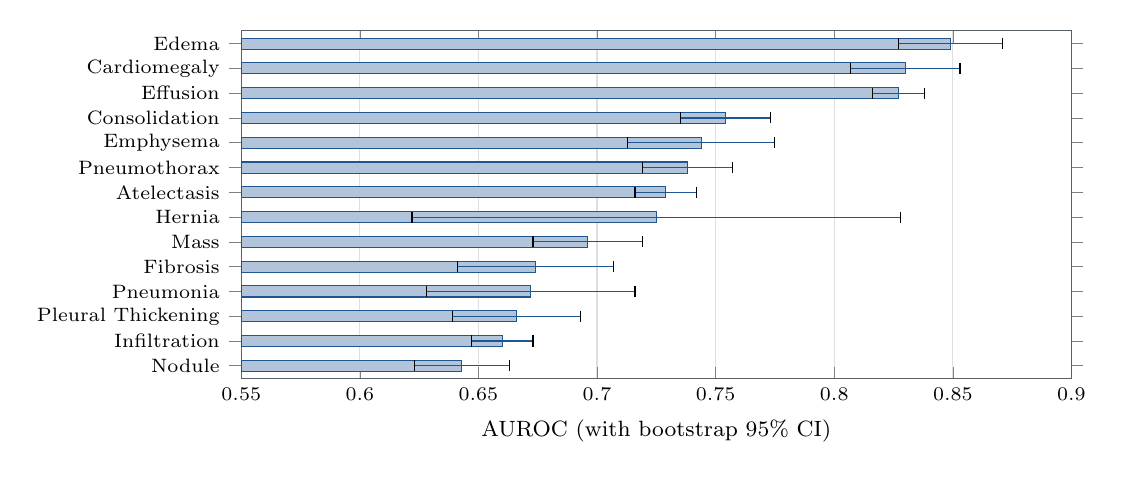
\begin{tikzpicture}
\begin{axis}[
  width=\linewidth, height=6.0cm,
  xbar, xmin=0.55, xmax=0.90,
  bar width=4.0pt,
  enlarge y limits=0.04,
  symbolic y coords={Nodule,Infiltration,Pleural Thickening,Pneumonia,Fibrosis,
    Mass,Hernia,Atelectasis,Pneumothorax,Emphysema,Consolidation,Effusion,
    Cardiomegaly,Edema},
  ytick=data,
  xlabel={AUROC (with bootstrap 95\% CI)},
  xmajorgrids, grid style={gray!25},
  tick label style={font=\scriptsize},
  label style={font=\footnotesize},
  axis line style={mirrorgray},
]
\addplot[fill=mirrorblue!35, draw=mirrorblue, error bars/.cd,
         x dir=both, x explicit] coordinates {
  (0.643,Nodule)             +- (0.020,0)
  (0.660,Infiltration)       +- (0.013,0)
  (0.666,Pleural Thickening) +- (0.027,0)
  (0.672,Pneumonia)          +- (0.044,0)
  (0.674,Fibrosis)           +- (0.033,0)
  (0.696,Mass)               +- (0.023,0)
  (0.725,Hernia)             +- (0.103,0)
  (0.729,Atelectasis)        +- (0.013,0)
  (0.738,Pneumothorax)       +- (0.019,0)
  (0.744,Emphysema)          +- (0.031,0)
  (0.754,Consolidation)      +- (0.019,0)
  (0.827,Effusion)           +- (0.011,0)
  (0.830,Cardiomegaly)       +- (0.023,0)
  (0.849,Edema)              +- (0.022,0)
};
\end{axis}
\end{tikzpicture}
\caption{Per-label test AUROC on ChestMNIST (DenseNet-121, $64$\,px source
upsampled to $224$\,px, CPU, best of four epochs, $N_{\text{test}}{=}12{,}000$),
with bootstrap $95\%$ CI whiskers, sorted ascending. The ordering tracks how
visible each finding is, and every interval clears the $0.5$ chance line.}
\label{fig:cxr-auroc}
\end{figure}

\subsection{The operating point: silence on most of the taxonomy}
\label{sec:operating}
AUROC is threshold-free, and it hides what this model does when asked for a
decision. At the default $0.5$ threshold, \textbf{11 of the 14 labels never
produce a single positive prediction} across all $12{,}000$ test studies: their
sensitivity is exactly $0.0$, their specificity exactly $1.0$, and their PPV
undefined (Table~\ref{tab:operating}). The three that fire at all are Effusion,
Infiltration, and Pneumothorax, and Pneumothorax fires on $1.2\%$ of its positive
cases. Macro sensitivity is $0.019$ and macro F1 is $0.031$.

This is not a conservative operating point chosen for a clinical reason. Nothing
was tuned: $0.5$ is the default, and under prevalences from $17.5\%$
(Infiltration) down to $0.2\%$ (Hernia) a lightly trained model minimizes its loss
by pushing almost every output below it. At this threshold the classifier is not
usable as a detector. That is a property of the training budget and the destroyed
resolution, not a design decision, and the AUROC of Section~\ref{sec:chestmnist}
should be read as a statement about \emph{ranking} that carries no implication
about decisions.

\begin{table}[tbp]
\centering
\caption{Operating point at the default $0.5$ threshold ($N=12{,}000$).
Prevalence is $\text{support}_{+}/N$. Eleven labels (Atelectasis, Cardiomegaly,
Mass, Nodule, Pneumonia, Consolidation, Edema, Emphysema, Fibrosis, Pleural
Thickening, Hernia) emit no positive prediction at all, so their PPV is
undefined.}
\label{tab:operating}
\footnotesize
\begin{tabular}{@{}lcccc@{}}
\toprule
\textbf{Label} & \textbf{Prev.} & \textbf{Sens.} & \textbf{Spec.} & \textbf{PPV} \\
\midrule
Effusion            & 0.121 & 0.143 & 0.987 & 0.599 \\
Infiltration        & 0.175 & 0.110 & 0.967 & 0.415 \\
Pneumothorax        & 0.049 & 0.012 & 0.999 & 0.350 \\
The other 11 labels & 0.002--0.109 & 0.000 & 1.000 & --- \\
\midrule
Macro (all 14)      &       & 0.019 & 0.997 & 0.097 \\
\bottomrule
\end{tabular}
\end{table}

\subsection{Calibration against a no-skill baseline}
\label{sec:calib}
Read on their own, the calibration numbers look strong: macro Brier $0.045$ and
ECE $0.018$. They are also close to meaningless here, and the arithmetic showing
it needs no new experiment. For a label with prevalence $p$, a constant predictor
that ignores the image and always returns $p$ achieves a Brier score of exactly
$p(1-p)$. Averaged over the 14 ChestMNIST prevalences, that is a macro Brier of
$\mathbf{0.0472}$ for a model that has learned nothing at all. Our trained
classifier scores $\mathbf{0.0453}$. The entire measured calibration advantage of
a DenseNet-121 over a constant is $0.0019$ Brier, about $4\%$.

We report this as a finding rather than an embarrassment, because it generalizes
past our model. Under the class imbalance typical of multi-label radiology, where
most labels sit below $5\%$ prevalence, $p(1-p)$ is small for almost every label,
so the no-skill floor of the aggregate metric is already low and there is little
room between it and a perfect score. A model silent on 11 of 14 labels still posts
a Brier of $0.045$ and an ECE of $0.018$, numbers that would pass unremarked in
most results tables. Aggregate calibration metrics on imbalanced multi-label
medical tasks should be reported against the constant-prevalence baseline, or not
offered as evidence of quality at all.

\subsection{Harness control on synthetic data}
\label{sec:synthetic}
To check that the training and scoring machinery credits only real signal, we
train the same pipeline on a synthetic dataset whose generator injects a visible
blob for seven of the fourteen labels and leaves the other seven with no visual
correlate. A correct harness should learn the first group and sit near chance on
the second, and it does: the seven signal-bearing labels reach a mean AUROC of
$0.917$ (Mass $0.979$ down to Edema $0.866$) and the seven no-signal labels
average $0.533$ (Hernia $0.620$ down to Pleural Thickening $0.434$). The no-signal
mean sits slightly above $0.5$ rather than on it, which is what a finite
$350$-image test split should give, and the individual no-signal labels straddle
chance in both directions. The separation is what the control is for: the
classifier, loss, metrics, and bootstrap intervals respond to injected signal and
not to label frequency or ordering, so nothing is leaking.

\subsection{Post-hoc invariance and latency}
\label{sec:ablation}
Layers 2 and 3 run after the forward pass and modify no weights and no logits, so
the predictions are identical across the three conditions by construction. The
harness confirms it: the maximum per-label probability change against the
classification-only baseline is $0.000$ over $n{=}24$ studies. This is a
regression test, not a result. It earns its place because a nonzero delta would
expose a real bug, an accidental coupling between the layers.

The cost that does vary is latency (Table~\ref{tab:ablation}). Prediction takes
about $100$~ms per study on CPU, the Grad-CAM pass adds $36$ to $41$~ms, and the
offline template report adds $0.03$~ms. The two conditions that run Grad-CAM
measured $41.4$ and $36.2$~ms for the same work, which is the run-to-run spread of
a 24-study CPU profile and is why the full-pipeline total ($136$~ms) came in below
the localization-only total ($141$~ms). The test suite asserts the same invariance
per modality against stubbed backbones, so the property is structural rather than
particular to the chest checkpoint; no brain-MRI or head-CT measurement exists
because no such checkpoint does.

\begin{table*}[tp]
\centering
\caption{Ablation conditions with measured per-stage latency (DenseNet-121 on
ChestMNIST, profiled over $24$ studies on CPU). \textbf{There is one AUROC
measurement here, not three.} Macro AUROC $=0.729$ is the single value from
Section~\ref{sec:chestmnist}; it applies unchanged to every row because the
post-hoc layers cannot alter a prediction, and the harness copies it into each row
for that reason. The measurements that differ between rows are the latencies; the
measurement verifying the rows are comparable is the probability delta.}
\label{tab:ablation}
\footnotesize
\begin{tabular}{@{}lcccr@{}}
\toprule
\textbf{Condition} & \textbf{Classify} & \textbf{Localize} & \textbf{Report} & \textbf{Latency (ms/study)} \\
\midrule
Classification only       & \checkmark &            &            & \phantom{$+$}101 \ (prediction), total 101 \\
$+$ Evidence localization & \checkmark & \checkmark &            & $+$41 \ (Grad-CAM), total 141 \\
Full MIRROR               & \checkmark & \checkmark & \checkmark & $+$0.03 \ (template report), total 136 \\
\midrule
\multicolumn{5}{@{}l}{Macro AUROC $=0.729$ for all three rows (one measurement, $N_{\text{test}}=12{,}000$).} \\
\multicolumn{5}{@{}l}{Maximum per-label probability change vs.\ the baseline $=0.000$ over $n=24$ studies.} \\
\bottomrule
\end{tabular}
\end{table*}

\begin{figure}[tbp]
\centering
\begin{minipage}[t]{0.47\linewidth}
\centering
\figorbox{figures/overlay-consolidation.png}{\linewidth}{Grad-CAM overlay}
\\[2pt]{\scriptsize (a) Evidence localization}
\end{minipage}\hspace{0.03\linewidth}%
\begin{minipage}[t]{0.47\linewidth}
\centering
\figorbox{figures/report-findings.png}{\linewidth}{Draft report}
\\[2pt]{\scriptsize (b) Draft report}
\end{minipage}
\caption{One study end to end on the \textbf{hosted serverless engine} (a vision
LLM reading the image directly), not the benchmarked local stack. (b) is the
worked example of Section~\ref{sec:ethics}: alongside its grounded findings the
report states a cardiothoracic ratio and clear costophrenic angles, neither of
which any component of the system measured.}
\label{fig:qual}
\end{figure}

% -----------------------------------------------------------------------------
\section{Discussion}
\label{sec:discussion}

\paragraph{Finding-level grounding is a real guarantee and a narrow one.} The
useful thing MIRROR demonstrates is a boundary, and stating it precisely is worth
more than the classifier behind it. Because the language layer receives a label, a
probability, and a region name rather than an image, the set of findings the
report may assert is exactly the set the classifier produced. That is checkable
without trusting anything about the model: a reader holding the report and the
probability vector can verify the correspondence, and a test can assert it. It is
also strictly a claim about \emph{which findings appear}, and says nothing about
the sentences around them. A report that correctly asserts consolidation may frame
it with clauses the system never computed, and those clauses inherit the
credibility of the finding they sit beside (Section~\ref{sec:ethics}). This
distinction is the thing worth taking from the system, and architectures that
constrain only the former should say so rather than claiming groundedness
generally.

\paragraph{Where this stands against Rudin.} MIRROR is precisely the architecture
Rudin~\cite{rudin2019stop} argues against for high-stakes decisions: an opaque CNN
with a saliency map and a language layer attached after the fact. We have no
rebuttal, and we do not claim the saliency map is faithful; the sanity checks of
Adebayo et al.~\cite{adebayo2018sanity} are the right instrument for testing that
and we have not run them. What we claim is narrower and does not depend on the
heatmap being faithful at all: the finding set is auditable, because a reader can
check the report against the probability vector directly. That is a retreat from
explanation to auditability, and we would rather name it than dress it up. An
inherently interpretable classifier would be the stronger answer.

\paragraph{On measuring the wrong thing.} The ChestMNIST result is a systems
demonstration: a real classifier, trained and scored end to end, whose per-label
ordering tracks radiographic visibility and whose intervals clear chance. It is
also unusable at its own default threshold, and the sequence of numbers it
produces is instructive. AUROC $0.729$ reads as a modest but working model. Brier
$0.045$ and ECE $0.018$ read as a well-calibrated one. Both are true, and a model
that emits no positive prediction for 11 of 14 labels sits behind them. Only the
operating point exposes that, which argues for reporting sensitivity and PPV
alongside every AUROC in this literature, and calibration against a prevalence
baseline rather than on an absolute scale. Separately, serving one contract from
both a PyTorch stack and a hosted vision LLM shows the \emph{interface} MIRROR
proposes is independent of the backend, at the price of the asymmetry in
Section~\ref{sec:serving}: the grounding guarantee belongs to the local stack,
not to the deployed website.

% -----------------------------------------------------------------------------
\section{Ethics, Safety, and Limitations}
\label{sec:ethics}

\textbf{Not a medical device.} MIRROR is a research prototype, not reviewed or
cleared by any regulatory body; every output is a draft that must be verified by a
licensed radiologist and must not be used for diagnosis or treatment. Each report
carries that disclaimer explicitly.

\textbf{A worked example of ungrounded detail.} Fig.~\ref{fig:qual} shows a
generated report beside its evidence overlay. Two phrases in it are worth quoting:
the cardiac silhouette is described as normal \emph{with a cardiothoracic ratio
below $0.5$}, and the \emph{costophrenic angles are noted to be clear}. The system
measured neither. No cardiothoracic ratio was computed, no cardiac or thoracic
boundary was segmented, and no costophrenic angle was localized; the pipeline
produced 14 probabilities and up to three saliency centroids, and nothing in that
evidence supports either clause. Both are fluent radiology register generated to
fill out a report. They also sit in the same paragraph as assertions that
\emph{are} grounded, and that adjacency is the danger: a reader who checks the
consolidation finding against the overlay and finds it correct has been given a
reason to extend trust to the sentence beside it. Fluency makes ungrounded detail
more dangerous rather than less, because it arrives wearing the credibility of the
verified finding next to it. This is why finding-level grounding cannot be
described as making a report safe, and why the AI-generated-draft disclaimer is
load-bearing rather than boilerplate.

\textbf{Human subjects and data governance.} No ethics-board review was required:
this work uses only existing, public, de-identified benchmark datasets (NIH
ChestX-ray14 and its MedMNIST derivative) and collects no new data from human
subjects. Those datasets are governed by their own data use agreements; no raw
images, weights, or protected health information are committed to version control,
and the DICOM ingest extracts only non-PHI technical tags.

\textbf{Limitations.} Our one quantitative benchmark is ChestMNIST, at $64$-pixel
source resolution on a $7{,}200$-image budget, and at its default threshold the
classifier is not a working detector (Section~\ref{sec:operating}). No clinical
claim of any kind follows from it. Multi-modality is architectural: the brain-MRI
and head-CT paths are implemented and exercised by the test suite but have no
trained checkpoints, so MIRROR makes no predictive claim on those modalities.
Explanation quality is unmeasured: the pointing-game and IoU protocol is
implemented but not run, and no reader study has been conducted, so we have no
evidence that the localization or report layers help a human, only that they cost
about $40$~ms. Class-activation maps are coarse and can highlight context rather
than lesion~\cite{adebayo2018sanity}, and we have not run the sanity checks that
would detect it. The $3\times3$ location grid is a deliberately coarse descriptor.
Report quality is assessed only qualitatively; a comparison against real
radiologist reports (for example MIMIC-CXR~\cite{johnson2019mimiccxr}) is future
work.

% -----------------------------------------------------------------------------
\section{Conclusion}

MIRROR composes classification, evidence localization, and report generation into
one traceable, registry-driven pipeline, and the property worth carrying forward
is a boundary rather than a score: constraining the language layer to structured
evidence makes the \emph{finding set} of a report auditable and does nothing for
the prose around it. On ChestMNIST the classifier reaches macro AUROC $0.729$ with
a per-label ordering that tracks visibility, and at its default threshold it emits
no positive prediction for 11 of its 14 labels while still posting a Brier score
within $0.002$ of a constant-prevalence predictor. We report that pair together
deliberately: it is the clearest evidence we produced that aggregate metrics on
imbalanced multi-label tasks can look healthy over a model that does nothing. Next
steps are full-resolution training, the saliency sanity checks we cite but did not
run, and a reader study, which is the only thing that would test whether any of
this helps a radiologist.

% -----------------------------------------------------------------------------
\section*{Reproducibility}
\footnotesize
Code: \url{https://github.com/vignesh-nagarajan-vn/MIRROR}. Live demo (hosted
engine): \url{https://mirror-ten-jet.vercel.app/}. A zero-setup CLI demo
(\code{python -m demo.run\_demo <image>}) runs the local pipeline on ImageNet
weights with the offline template backend, no checkpoint or key required. Every
results JSON stamps a \code{reproducibility} block (seed, git commit, library
versions), and the unit tests are torch-free. The ChestMNIST result
(\code{configs/chestmnist.yaml}) and the synthetic control regenerate from seed
$42$; outputs are committed under \code{results/}, and the no-skill baseline of
Section~\ref{sec:calib} is recomputed from that JSON by
\code{paper/calibration\_baseline.py}.

% -----------------------------------------------------------------------------
\section*{Acknowledgments}
\small
This work was completed as part of the Global Indian Scientists \& Technocrats
(GIST) 2026 Summer Research Internship. The author thanks his mentor,
\textbf{Sriram Venkatapathy}, an Applied AI Researcher at Capital One who holds a
PhD in Computer Science from the Indian Institute of Technology (IIT) Hyderabad,
for his guidance throughout the project: his experience building and evaluating
machine-learning systems in industry shaped both the architecture and the
emphasis on measurable, reproducible evaluation.

% -----------------------------------------------------------------------------
\section*{Declarations}
\footnotesize
\textbf{Data availability:} all datasets used are public, namely NIH ChestX-ray14
and its MedMNIST derivative ChestMNIST (CC~BY~4.0); code, configurations, and result
files are in the repository linked above. \textbf{Competing interests:} the author
declares none. \textbf{Funding:} this work received no external research funding and
was conducted as part of the GIST 2026 Summer Research Internship.

% =============================================================================
%  Bibliography embedded so this stays a single, self-contained file (one
%  pdfLaTeX pass, no bibtex). PENDING before camera-ready: verify page numbers /
%  venue strings against each paper's official record.
% =============================================================================
\begin{thebibliography}{99}
\scriptsize
\setlength{\itemsep}{1pt}
\setlength{\parsep}{0pt}

\bibitem{wang2017chestxray}
X.~Wang, Y.~Peng, L.~Lu, Z.~Lu, M.~Bagheri, and R.~M. Summers.
ChestX-ray8: Hospital-scale chest X-ray database and benchmarks on
weakly-supervised classification and localization of common thorax diseases.
\emph{CVPR}, 2097--2106, 2017.

\bibitem{rajpurkar2017chexnet}
P.~Rajpurkar, J.~Irvin, K.~Zhu, et~al.
CheXNet: Radiologist-level pneumonia detection on chest X-rays with deep learning.
\emph{arXiv:1711.05225}, 2017.

\bibitem{johnson2019mimiccxr}
A.~E.~W. Johnson, T.~J. Pollard, S.~J. Berkowitz, et~al.
MIMIC-CXR, a de-identified publicly available database of chest radiographs with
free-text reports. \emph{Scientific Data}, 6(1):317, 2019.

\bibitem{yang2023medmnist}
J.~Yang, R.~Shi, D.~Wei, Z.~Liu, L.~Zhao, B.~Ke, H.~Pfister, and B.~Ni.
MedMNIST v2: A large-scale lightweight benchmark for 2D and 3D biomedical image
classification. \emph{Scientific Data}, 10(1):41, 2023.

\bibitem{huang2017densenet}
G.~Huang, Z.~Liu, L.~van~der~Maaten, and K.~Q. Weinberger.
Densely connected convolutional networks. \emph{CVPR}, 4700--4708, 2017.

\bibitem{tan2019efficientnet}
M.~Tan and Q.~V. Le.
EfficientNet: Rethinking model scaling for convolutional neural networks.
\emph{ICML}, 2019.

\bibitem{dosovitskiy2021vit}
A.~Dosovitskiy, L.~Beyer, A.~Kolesnikov, et~al.
An image is worth 16x16 words: Transformers for image recognition at scale.
\emph{ICLR}, 2021.

\bibitem{selvaraju2017gradcam}
R.~R. Selvaraju, M.~Cogswell, A.~Das, R.~Vedantam, D.~Parikh, and D.~Batra.
Grad-CAM: Visual explanations from deep networks via gradient-based localization.
\emph{ICCV}, 618--626, 2017.

\bibitem{wang2020scorecam}
H.~Wang, Z.~Wang, M.~Du, et~al.
Score-CAM: Score-weighted visual explanations for convolutional neural networks.
\emph{CVPR Workshops}, 2020.

\bibitem{zhang2016pointing}
J.~Zhang, S.~A. Bargal, Z.~Lin, J.~Brandt, X.~Shen, and S.~Sclaroff.
Top-down neural attention by excitation backprop. \emph{ECCV}, 2016.

\bibitem{adebayo2018sanity}
J.~Adebayo, J.~Gilmer, M.~Muelly, I.~Goodfellow, M.~Hardt, and B.~Kim.
Sanity checks for saliency maps. \emph{NeurIPS}, 2018.

\bibitem{rudin2019stop}
C.~Rudin.
Stop explaining black box machine learning models for high stakes decisions and
use interpretable models instead. \emph{Nature Machine Intelligence},
1(5):206--215, 2019.

\bibitem{wang2018tienet}
X.~Wang, Y.~Peng, L.~Lu, Z.~Lu, and R.~M. Summers.
TieNet: Text-image embedding network for common thorax disease classification and
reporting in chest X-rays. \emph{CVPR}, 2018.

\bibitem{chen2020r2gen}
Z.~Chen, Y.~Song, T.-H. Chang, and X.~Wan.
Generating radiology reports via memory-driven transformer. \emph{EMNLP}, 2020.

\bibitem{liu2019clinically}
G.~Liu, T.-M.~H. Hsu, M.~McDermott, et~al.
Clinically accurate chest X-ray report generation. \emph{MLHC}, 2019.

\bibitem{tjoa2021survey}
E.~Tjoa and C.~Guan.
A survey on explainable artificial intelligence (XAI): Toward medical XAI.
\emph{IEEE TNNLS}, 32(11):4793--4813, 2021.

\end{thebibliography}

\end{document}
